% Options for packages loaded elsewhere
% Options for packages loaded elsewhere
\PassOptionsToPackage{unicode}{hyperref}
\PassOptionsToPackage{hyphens}{url}
\PassOptionsToPackage{dvipsnames,svgnames,x11names}{xcolor}
%
\documentclass[
  portuguese,
  letterpaper,
  DIV=11,
  numbers=noendperiod]{scrreprt}
\usepackage{xcolor}
\usepackage{amsmath,amssymb}
\setcounter{secnumdepth}{5}
\usepackage{iftex}
\ifPDFTeX
  \usepackage[T1]{fontenc}
  \usepackage[utf8]{inputenc}
  \usepackage{textcomp} % provide euro and other symbols
\else % if luatex or xetex
  \usepackage{unicode-math} % this also loads fontspec
  \defaultfontfeatures{Scale=MatchLowercase}
  \defaultfontfeatures[\rmfamily]{Ligatures=TeX,Scale=1}
\fi
\usepackage{lmodern}
\ifPDFTeX\else
  % xetex/luatex font selection
\fi
% Use upquote if available, for straight quotes in verbatim environments
\IfFileExists{upquote.sty}{\usepackage{upquote}}{}
\IfFileExists{microtype.sty}{% use microtype if available
  \usepackage[]{microtype}
  \UseMicrotypeSet[protrusion]{basicmath} % disable protrusion for tt fonts
}{}
\makeatletter
\@ifundefined{KOMAClassName}{% if non-KOMA class
  \IfFileExists{parskip.sty}{%
    \usepackage{parskip}
  }{% else
    \setlength{\parindent}{0pt}
    \setlength{\parskip}{6pt plus 2pt minus 1pt}}
}{% if KOMA class
  \KOMAoptions{parskip=half}}
\makeatother
% Make \paragraph and \subparagraph free-standing
\makeatletter
\ifx\paragraph\undefined\else
  \let\oldparagraph\paragraph
  \renewcommand{\paragraph}{
    \@ifstar
      \xxxParagraphStar
      \xxxParagraphNoStar
  }
  \newcommand{\xxxParagraphStar}[1]{\oldparagraph*{#1}\mbox{}}
  \newcommand{\xxxParagraphNoStar}[1]{\oldparagraph{#1}\mbox{}}
\fi
\ifx\subparagraph\undefined\else
  \let\oldsubparagraph\subparagraph
  \renewcommand{\subparagraph}{
    \@ifstar
      \xxxSubParagraphStar
      \xxxSubParagraphNoStar
  }
  \newcommand{\xxxSubParagraphStar}[1]{\oldsubparagraph*{#1}\mbox{}}
  \newcommand{\xxxSubParagraphNoStar}[1]{\oldsubparagraph{#1}\mbox{}}
\fi
\makeatother

\usepackage{color}
\usepackage{fancyvrb}
\newcommand{\VerbBar}{|}
\newcommand{\VERB}{\Verb[commandchars=\\\{\}]}
\DefineVerbatimEnvironment{Highlighting}{Verbatim}{commandchars=\\\{\}}
% Add ',fontsize=\small' for more characters per line
\usepackage{framed}
\definecolor{shadecolor}{RGB}{241,243,245}
\newenvironment{Shaded}{\begin{snugshade}}{\end{snugshade}}
\newcommand{\AlertTok}[1]{\textcolor[rgb]{0.68,0.00,0.00}{#1}}
\newcommand{\AnnotationTok}[1]{\textcolor[rgb]{0.37,0.37,0.37}{#1}}
\newcommand{\AttributeTok}[1]{\textcolor[rgb]{0.40,0.45,0.13}{#1}}
\newcommand{\BaseNTok}[1]{\textcolor[rgb]{0.68,0.00,0.00}{#1}}
\newcommand{\BuiltInTok}[1]{\textcolor[rgb]{0.00,0.23,0.31}{#1}}
\newcommand{\CharTok}[1]{\textcolor[rgb]{0.13,0.47,0.30}{#1}}
\newcommand{\CommentTok}[1]{\textcolor[rgb]{0.37,0.37,0.37}{#1}}
\newcommand{\CommentVarTok}[1]{\textcolor[rgb]{0.37,0.37,0.37}{\textit{#1}}}
\newcommand{\ConstantTok}[1]{\textcolor[rgb]{0.56,0.35,0.01}{#1}}
\newcommand{\ControlFlowTok}[1]{\textcolor[rgb]{0.00,0.23,0.31}{\textbf{#1}}}
\newcommand{\DataTypeTok}[1]{\textcolor[rgb]{0.68,0.00,0.00}{#1}}
\newcommand{\DecValTok}[1]{\textcolor[rgb]{0.68,0.00,0.00}{#1}}
\newcommand{\DocumentationTok}[1]{\textcolor[rgb]{0.37,0.37,0.37}{\textit{#1}}}
\newcommand{\ErrorTok}[1]{\textcolor[rgb]{0.68,0.00,0.00}{#1}}
\newcommand{\ExtensionTok}[1]{\textcolor[rgb]{0.00,0.23,0.31}{#1}}
\newcommand{\FloatTok}[1]{\textcolor[rgb]{0.68,0.00,0.00}{#1}}
\newcommand{\FunctionTok}[1]{\textcolor[rgb]{0.28,0.35,0.67}{#1}}
\newcommand{\ImportTok}[1]{\textcolor[rgb]{0.00,0.46,0.62}{#1}}
\newcommand{\InformationTok}[1]{\textcolor[rgb]{0.37,0.37,0.37}{#1}}
\newcommand{\KeywordTok}[1]{\textcolor[rgb]{0.00,0.23,0.31}{\textbf{#1}}}
\newcommand{\NormalTok}[1]{\textcolor[rgb]{0.00,0.23,0.31}{#1}}
\newcommand{\OperatorTok}[1]{\textcolor[rgb]{0.37,0.37,0.37}{#1}}
\newcommand{\OtherTok}[1]{\textcolor[rgb]{0.00,0.23,0.31}{#1}}
\newcommand{\PreprocessorTok}[1]{\textcolor[rgb]{0.68,0.00,0.00}{#1}}
\newcommand{\RegionMarkerTok}[1]{\textcolor[rgb]{0.00,0.23,0.31}{#1}}
\newcommand{\SpecialCharTok}[1]{\textcolor[rgb]{0.37,0.37,0.37}{#1}}
\newcommand{\SpecialStringTok}[1]{\textcolor[rgb]{0.13,0.47,0.30}{#1}}
\newcommand{\StringTok}[1]{\textcolor[rgb]{0.13,0.47,0.30}{#1}}
\newcommand{\VariableTok}[1]{\textcolor[rgb]{0.07,0.07,0.07}{#1}}
\newcommand{\VerbatimStringTok}[1]{\textcolor[rgb]{0.13,0.47,0.30}{#1}}
\newcommand{\WarningTok}[1]{\textcolor[rgb]{0.37,0.37,0.37}{\textit{#1}}}

\usepackage{longtable,booktabs,array}
\usepackage{calc} % for calculating minipage widths
% Correct order of tables after \paragraph or \subparagraph
\usepackage{etoolbox}
\makeatletter
\patchcmd\longtable{\par}{\if@noskipsec\mbox{}\fi\par}{}{}
\makeatother
% Allow footnotes in longtable head/foot
\IfFileExists{footnotehyper.sty}{\usepackage{footnotehyper}}{\usepackage{footnote}}
\makesavenoteenv{longtable}
\usepackage{graphicx}
\makeatletter
\newsavebox\pandoc@box
\newcommand*\pandocbounded[1]{% scales image to fit in text height/width
  \sbox\pandoc@box{#1}%
  \Gscale@div\@tempa{\textheight}{\dimexpr\ht\pandoc@box+\dp\pandoc@box\relax}%
  \Gscale@div\@tempb{\linewidth}{\wd\pandoc@box}%
  \ifdim\@tempb\p@<\@tempa\p@\let\@tempa\@tempb\fi% select the smaller of both
  \ifdim\@tempa\p@<\p@\scalebox{\@tempa}{\usebox\pandoc@box}%
  \else\usebox{\pandoc@box}%
  \fi%
}
% Set default figure placement to htbp
\def\fps@figure{htbp}
\makeatother



\ifLuaTeX
\usepackage[bidi=basic]{babel}
\else
\usepackage[bidi=default]{babel}
\fi
% get rid of language-specific shorthands (see #6817):
\let\LanguageShortHands\languageshorthands
\def\languageshorthands#1{}


\setlength{\emergencystretch}{3em} % prevent overfull lines

\providecommand{\tightlist}{%
  \setlength{\itemsep}{0pt}\setlength{\parskip}{0pt}}



 


<style>
   /* ===== largura máxima do conteúdo ===== */
  :root { --content-max-width: 1600px; }

  /* ===== cores utilitárias (suas classes) ===== */
  .red  { color: #e53935; }
  .blue { color: dodgerblue; }
  .darkblue  { color: #003366; }   /* azul escuro */
  .darkgreen { color: #006400; }   /* verde escuro */
  .orange    { color: #ff8c00; }   /* laranja */
  .purple    { color: #800080; }   /* roxo */
  .note { color:#6f42c1; background:#f3e8ff; padding:2px 6px; border-radius:6px; }

  /* ===== BOTÃO CENTRAL personalizável ===== */
  #qst-centered {
    position: fixed;
    top: 12px;
    left: 50%;
    transform: translateX(-50%);
    z-index: 1031;
    display: inline-flex;
    align-items: center;
    justify-content: center;
    width: 36px;
    height: 36px;
    border-radius: 999px;
    background: #fff;
    border: 1px solid #e6ecf3;
    box-shadow: 0 2px 8px rgba(0,0,0,.08);
    cursor: pointer;
  }
  #qst-centered:hover {
    box-shadow: 0 3px 12px rgba(0,0,0,.12);
    border-color: #d8e2ef;
  }
  #qst-centered .qst-bar {
    width: 18px; height: 2px; background:#333; margin: 2px 0;
  }

  /* Em telas pequenas, deixe o comportamento padrão do tema */
  @media (max-width: 991.98px){
    #qst-centered { display: none; }
  }

  /* Evitar que o botão sobreponha o H1 ao navegar por âncoras */
  .content h1.title, .content h1 { scroll-margin-top: 60px; }
</style>



<script>
  document.addEventListener('DOMContentLoaded', function () {
    // 1) Verifique se o include carregou: deve haver o quadradinho verde no canto (body::after)
    // 2) Criar um botão central próprio (independente do botão do tema)
    if (!document.getElementById('qst-centered')) {
      const b = document.createElement('button');
      b.id = 'qst-centered';
      b.setAttribute('type','button');
      b.setAttribute('title','Mostrar/ocultar barra lateral');

      for (let i=0;i<3;i++){
        const bar = document.createElement('div');
        bar.className = 'qst-bar';
        b.appendChild(bar);
      }
      document.body.appendChild(b);

      // Handler do clique: alterna o estado do sidebar usando Bootstrap Collapse
      b.addEventListener('click', () => {
        try {
          const sidebar = document.querySelector('#quarto-sidebar');
          const body = document.body;

          // alterna uma classe no body (útil para temas que usam isso)
          body.classList.toggle('sidebar-collapsed');

          if (sidebar) {
            // se estiver colapsado, mostramos; se estiver aberto, escondemos
            const isOpen = sidebar.classList.contains('show');
            // tenta usar a API do Bootstrap, se estiver presente
            const bs = (window.bootstrap && window.bootstrap.Collapse)
              ? window.bootstrap.Collapse.getOrCreateInstance(sidebar)
              : null;

            if (bs) {
              if (isOpen) { bs.hide(); } else { bs.show(); }
            } else {
              // fallback: alterna class "show" manualmente
              sidebar.classList.toggle('show');
            }

            // mantém a classe do body coerente
            if (sidebar.classList.contains('show')) {
              body.classList.remove('sidebar-collapsed');
            } else {
              body.classList.add('sidebar-collapsed');
            }
          }
        } catch (e) {
          console.warn('Toggle central falhou:', e);
        }
      });
    }
  });
</script>
<script>
  (function(){
    function pickVisible(el){ return el && el.offsetParent !== null; }

    function findNativeToggle(){
      // 1) seletores “clássicos” do Quarto (cobrindo variações)
      const sels = [
        '#quarto-sidebar-toggle',
        '.quarto-sidebar-toggle',
        'button.sidebar-toggle',
        'button[aria-controls="quarto-sidebar"]',
        'a[aria-controls="quarto-sidebar"]',
        '[data-bs-target="#quarto-sidebar"]',
        '[aria-label*="sidebar" i]'
      ];
      for (const s of sels){
        const el = document.querySelector(s);
        if (pickVisible(el)) return el;
      }

      // 2) Heurística: procura um botão pequeno no canto sup. esquerdo
      const candidates = Array.from(document.querySelectorAll('button, a, .btn'));
      const ranked = candidates
        .map(el => [el, el.getBoundingClientRect()])
        .filter(([el, r]) => r.width > 20 && r.width < 64 && r.height > 20 && r.height < 64 && r.top >= 0 && r.top < 120 && r.left >= 0 && r.left < 140)
        .sort((a,b) => (a[1].top - b[1].top) || (a[1].left - b[1].left));
      return ranked.length ? ranked[0][0] : null;
    }

    function moveNativeToggle(){
      const btn = findNativeToggle();
      if (!btn) return;

      // reposiciona o PRÓPRIO botão nativo
      btn.style.position   = 'fixed';
      btn.style.left       = '50%';
      btn.style.top        = '12px';
      btn.style.transform  = 'translateX(-50%)';
      btn.style.zIndex     = '1060';

      // estética opcional (remova se quiser o padrão do tema)
      btn.style.background = '#fff';
      btn.style.border     = '1px solid #e6ecf3';
      btn.style.boxShadow  = '0 2px 8px rgba(0,0,0,.08)';
      btn.style.borderRadius = '999px';
      btn.style.width      = '36px';
      btn.style.height     = '36px';
      btn.style.display    = 'inline-flex';
      btn.style.alignItems = 'center';
      btn.style.justifyContent = 'center';
      btn.style.padding    = '0';
    }

    function wire(){
      moveNativeToggle();
      // se o DOM mudar (p.ex. render tardio), tentamos de novo
      const obs = new MutationObserver(() => moveNativeToggle());
      obs.observe(document.body, {childList:true, subtree:true});
      // também ao redimensionar
      window.addEventListener('resize', moveNativeToggle);
    }

    if (document.readyState === 'loading'){
      document.addEventListener('DOMContentLoaded', wire);
    } else {
      wire();
    }
  })();
</script>

<style>
  /* Esconde o botão nativo original no canto ESQUERDO em telas médias+,
     caso ele reapareça por algum motivo (opcional). */
  @media (min-width: 992px){
    .sidebar .quarto-sidebar-toggle,
    .sidebar #quarto-sidebar-toggle,
    .sidebar button.sidebar-toggle{ visibility:hidden !important; }
  }
  /* Em telas pequenas, deixe como está (botão no canto esq.) */
  @media (max-width: 991.98px){
    /* nada aqui: usamos o padrão do tema */
  }
</style>
<style>
  /* ===== LARGURA MENOR PARA SIDEBAR E TOC =====
     Aplica só em telas médias/grandes para não atrapalhar mobile */
  @media (min-width: 992px){

    /* (1) Se o seu Quarto expõe variáveis, use-as (fica mais limpo) */
    :root{
      --sidebar-width: 220px;            /* esquerda */
      --margin-sidebar-width: 240px;     /* TOC à direita */
    }

    /* (2) Fallback robusto (quando tema/versão não usa as variáveis) */
    #quarto-sidebar{
      width: var(--sidebar-width) !important;
    }
    /* alguns temas têm contêiner interno com largura própria */
    #quarto-sidebar .sidebar,
    #quarto-sidebar .sidebar-content,
    .sidebar.sidebar-navigation{
      width: var(--sidebar-width) !important;
      max-width: var(--sidebar-width) !important;
    }

    /* TOC / margin sidebar (direita) */
    #quarto-margin-sidebar{
      width: var(--margin-sidebar-width) !important;
    }
    .margin-sidebar{
      width: var(--margin-sidebar-width) !important;
      max-width: var(--margin-sidebar-width) !important;
    }

    /* (3) Diminui o espaço entre as 3 colunas (sidebar | conteúdo | TOC) */
    #quarto-content.page-columns{
      column-gap: 14px !important;  /* experimente 10–18px */
    }

    /* (4) Conteúdo central sem “colchões” extras */
    main.content{
      padding-left: 0 !important;
      padding-right: 0 !important;
    }

    /* (5) Só estética: o search acompanha a nova largura */
    #quarto-sidebar input.sidebar-search{
      width: 100% !important;
    }
  }
</style>
<style>
  /* ===== Preenche melhor a área central ===== */
  @media (min-width: 992px){

    /* use os mesmos valores que você já está usando
       para sidebar e TOC (ou deixe estes) */
    :root{
      --sidebar-width: 220px;
      --margin-sidebar-width: 240px;
    }

    /* gap entre colunas + “almofada” lateral de página (gutters) */
    :root{
      --lv-gap: 14px;       /* mesmo column-gap que você definiu */
      --lv-page-pad: 12px;  /* gutters externos (um de cada lado) */
    }

    /* Faz o track do conteúdo central ocupar todo o restante da tela */
    :root{
      --content-max-width: calc(
        100vw
        - var(--sidebar-width)
        - var(--margin-sidebar-width)
        - (2 * var(--lv-gap))
        - (2 * var(--lv-page-pad))
      ) !important;
    }

    /* Garante que o elemento não imponha um max-width menor */
    main.content{
      max-width: none !important;
      padding-left: 0 !important;
      padding-right: 0 !important;
    }

    /* Ajusta o espaçamento entre as 3 colunas */
    #quarto-content.page-columns{
      column-gap: var(--lv-gap) !important;
    }

    /* Opcional: controla os gutters externos (margens da página) */
    .page-columns{
      padding-left: var(--lv-page-pad) !important;
      padding-right: var(--lv-page-pad) !important;
    }
  }
</style>

<style>
  /* ===== Ajuste seguro de larguras sem redesenhar o grid ===== */
  @media (min-width: 992px){
    /* 1) larguras das colunas do Quarto */
    :root{
      /* sidebar (esquerda) e TOC (direita) */
      --sidebar-width:           220px;  /* ajuste aqui, ex: 200-240 */
      --margin-sidebar-width:    240px;  /* TOC; ajuste aqui, ex: 220-260 */

      /* largura máxima do conteúdo (miolo) — pode ser grande */
      --content-max-width:       2000px; /* evita “miolo” estreito */
    }

    /* 2) aplica os valores sem mexer no grid */
    #quarto-sidebar{
      width: var(--sidebar-width) !important;
      min-width: var(--sidebar-width) !important;
    }
    #quarto-margin-sidebar{
      width: var(--margin-sidebar-width) !important;
      min-width: var(--margin-sidebar-width) !important;
    }

    /* 3) respiro e liberação de largura no conteúdo */
    main.content{
      max-width: none !important;          /* ignora limites herdados */
      padding-left:  14px !important;      /* “respiro” interno */
      padding-right: 14px !important;
      overflow: visible !important;        /* não corta texto nas bordas */
      box-sizing: border-box !important;
    }

    /* 4) diminui o espaço entre colunas (sem trocar ordem) */
    #quarto-content.page-columns{
      column-gap: 14px !important;         /* ajuste: 10–16px */
    }
  }

  /* Em telas pequenas, deixa o padrão móvel */
  @media (max-width: 991.98px){
    main.content{
      padding-left: 12px !important;
      padding-right: 12px !important;
    }
  }
</style>
<style>
  /* espaçamento padrão entre parágrafos */
  .content p { 
    margin-top: 0;
    margin-bottom: 1.2rem;  /* aumente/diminua aqui */
    line-height: 1.55;      /* opcional: linhas mais arejadas */
  }

  /* um pouco mais de espaço quando um parágrafo vem logo após outro */
  .content p + p {
    margin-top: 0.8rem;
  }

  /* parágrafos dentro de callouts/listas costumam ser “apertados” */
  .callout p { margin-bottom: 0.8rem; }
  li p { margin-bottom: 0.6rem; }
</style>
<style>
  /* ===== Correções para telas pequenas (celular) ===== */
  @media (max-width: 991.98px){

    /* 1) Some com o TOC direito para liberar largura */
    #quarto-margin-sidebar{
      display: none !important;
    }

    /* 2) Garante respiro nas laterais e ocupa 100% da viewport */
    main.content{
      max-width: none !important;
      width: 100% !important;
      padding-left: 14px !important;
      padding-right: 14px !important;
      box-sizing: border-box !important;
    }

    /* 3) Evita “salto” de layout pelo gap das colunas */
    #quarto-content.page-columns{
      column-gap: 10px !important;
      max-width: 100vw !important;
    }

    /* 4) Impede qualquer scroll horizontal do site */
    html, body{
      overflow-x: hidden !important;
    }

    /* 5) Todo conteúdo embutido deve respeitar a largura da tela */
    img, video, canvas, svg{
      max-width: 100% !important;
      height: auto !important;
    }
    iframe{
      width: 100% !important;
      max-width: 100% !important;
      /* se seus iframes forem muito altos, pode usar um aspect-ratio: */
      /* aspect-ratio: 16 / 9; height: auto; */
    }

    /* 6) Código e tabelas: rolagem horizontal em vez de cortar texto */
    pre, code{
      white-space: pre-wrap !important;
      word-break: break-word !important;
    }
    pre code{
      white-space: pre-wrap !important;
    }
    .cell-output-display, .table-responsive, table{
      overflow-x: auto !important;
      display: block !important;
      max-width: 100% !important;
    }

    /* 7) Sidebar móvel: largura confortável como off-canvas */
    #quarto-sidebar{
      width: 86vw !important;         /* ajuste se quiser mais/menos */
      max-width: 420px !important;
    }
  }
</style>
\KOMAoption{captions}{tableheading}
\makeatletter
\@ifpackageloaded{bookmark}{}{\usepackage{bookmark}}
\makeatother
\makeatletter
\@ifpackageloaded{caption}{}{\usepackage{caption}}
\AtBeginDocument{%
\ifdefined\contentsname
  \renewcommand*\contentsname{Índice}
\else
  \newcommand\contentsname{Índice}
\fi
\ifdefined\listfigurename
  \renewcommand*\listfigurename{Lista de Figuras}
\else
  \newcommand\listfigurename{Lista de Figuras}
\fi
\ifdefined\listtablename
  \renewcommand*\listtablename{Lista de Tabelas}
\else
  \newcommand\listtablename{Lista de Tabelas}
\fi
\ifdefined\figurename
  \renewcommand*\figurename{Figura}
\else
  \newcommand\figurename{Figura}
\fi
\ifdefined\tablename
  \renewcommand*\tablename{Tabela}
\else
  \newcommand\tablename{Tabela}
\fi
}
\@ifpackageloaded{float}{}{\usepackage{float}}
\floatstyle{ruled}
\@ifundefined{c@chapter}{\newfloat{codelisting}{h}{lop}}{\newfloat{codelisting}{h}{lop}[chapter]}
\floatname{codelisting}{Listagem}
\newcommand*\listoflistings{\listof{codelisting}{Lista de Listagens}}
\makeatother
\makeatletter
\makeatother
\makeatletter
\@ifpackageloaded{caption}{}{\usepackage{caption}}
\@ifpackageloaded{subcaption}{}{\usepackage{subcaption}}
\makeatother
\usepackage{bookmark}
\IfFileExists{xurl.sty}{\usepackage{xurl}}{} % add URL line breaks if available
\urlstyle{same}
\hypersetup{
  pdftitle={Usando o JSPlotly},
  pdflang={pt},
  colorlinks=true,
  linkcolor={blue},
  filecolor={Maroon},
  citecolor={Blue},
  urlcolor={Blue},
  pdfcreator={LaTeX via pandoc}}


\title{Usando o JSPlotly}
\author{}
\date{}
\begin{document}
\maketitle

\renewcommand*\contentsname{Índice}
{
\hypersetup{linkcolor=}
\setcounter{tocdepth}{2}
\tableofcontents
}

\bookmarksetup{startatroot}

\chapter{Introdução}\label{introduuxe7uxe3o}

~~Este \emph{livro vivo} tem por objetivo apresentar-lhe de forma
prática a ferramenta \emph{JSPlotly}. Seguem os capítulos em construção.

\bookmarksetup{startatroot}

\chapter{O aplicativo}\label{o-aplicativo}

~~\emph{JSPlotly} é um aplicativo pra criar objetos virtuais de
aprendizagem. Com ele é possível criar gráficos 2D e 3D, tabelas,
diagramas, fluxogramas, realizar cálculos, produzir objetos
tridimensionais, animações, simulações, jogos, sonorização, objetos
multimídia (animação+som), e até prototipagem experimental (Arduino, por
ex).

~~Ainda que possibilite isso tudo (e um pouco mais\ldots), apresenta-se
como um pequeno arquivo HTML pra ser carregado em qualquer navegador de
internet. Assim, \emph{JSPlotly} não depende de sistema operacional
(Windows, Linux, Android, iOS) e nem de dispositivo (desktop, notebook,
tablet, celular). Por ser pequenino e com atributo HTML, pode-se
compartilhar o programa e o objetos produzidos por qualquer meio físico
ou digital, incluindo redes sociais.

~~O \emph{JSPlotly} é livre !!! Tanto pra baixar como para
personalizá-lo, como garantido por sua
\href{https://creativecommons.org/licenses/by-nc/4.0/}{licença CC BY-NC
4.0}. Assim, você pode utilizá-lo, copiá-lo, distribui-lo e mesmo
adaptá-lo para \emph{fins não comerciais}, desde que mencione o autor
original.

\subsection{\texorpdfstring{O site
\emph{Bioquanti}}{O site Bioquanti}}\label{o-site-bioquanti}

~~O aplicativo, suas características, seu modo de uso e \emph{mais de
uma centena de objetos de aprendizagem interativos} estão abertamente
disponíveis junto ao website
\href{https://bioquanti.netlify.app/}{Bioquanti}. O site é uma
iniciativa para propagar a ideia de se utilizar código de programação
voltados para a construção de objetos didáticos para conteúdos
curriculares, tanto para o ensino básico como para o ensino superior e
pesquisa científica. Numa \emph{``frasezinha''} de efeito: \emph{códigos
para conteúdos}.

~~O \emph{Bioquanti} foi desenhado para seu autoinstrucional, ou seja,
para que você consiga acompanhar o seu conteúdo e reproduzir/adaptar os
códigos para a construção de diversos tipos de objetos didáticos sem
necessitar de um(a) professor(a). Lá você encontrará tutoriais,
\emph{ebooks}, objetos didáticos interativos, códigos diversos, vídeos,
e intruções gerais para o uso de \emph{quatro programas} de distribuição
livre.

~~Esses programas são o \emph{JSPlotly}, para construção de objetos de
aprendizagem interativos variados, o \emph{Jmol} para visualização
tridimensional de moléculas, o \emph{R} e sua interface gráfica
\emph{RStudio} para tudo que possa pensar em ensino e pesquisa, e o
\emph{Sisma}, um programa feito na UNIFAL-MG para simular a dinâmica de
fluxos em um diagrama. Todos esses programas são livres, assim como
todos os materiais contidos no site. Veja uma imagem da página principal
do site abaixo.

\hfill\break

\begin{figure}

\centering{

\href{https://bioquanti.netlify.app/}{\pandocbounded{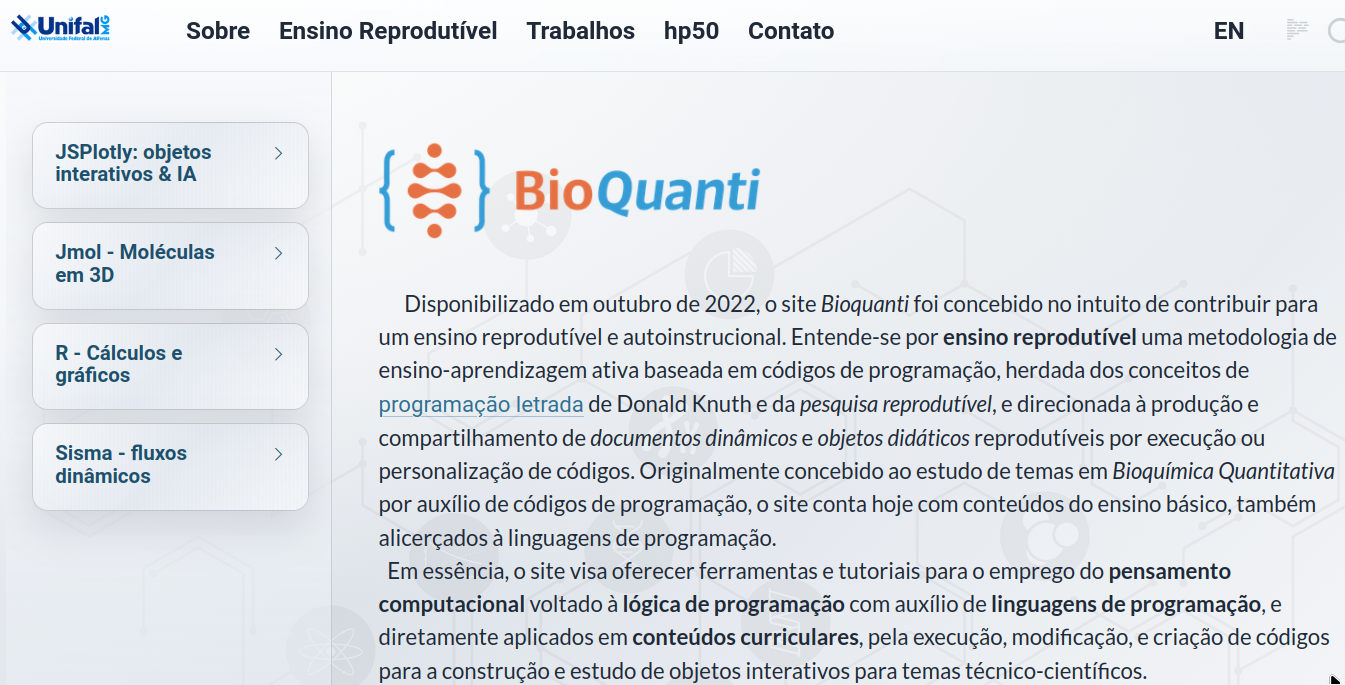
\includegraphics[keepaspectratio]{figs/bioquanti.png}}}

}

\caption{\label{fig-bioquanti}Página de visita do site Bioquanti,
apresentando uma barra lateral contendo acesso para 4 programas de livre
distribuição e materiais correlatos ao ensino e à pesquisa}

\end{figure}%

\hfill\break

\section{Botando a mão na massa !}\label{botando-a-muxe3o-na-massa}

\hfill\break

~~Agora, voltando ao \emph{JSPlotly}. Quer ver como é simples utilizá-lo
? Dê uma olhada na tela única do aplicativo abaixo.

\hfill\break

\begin{figure}

\centering{

\pandocbounded{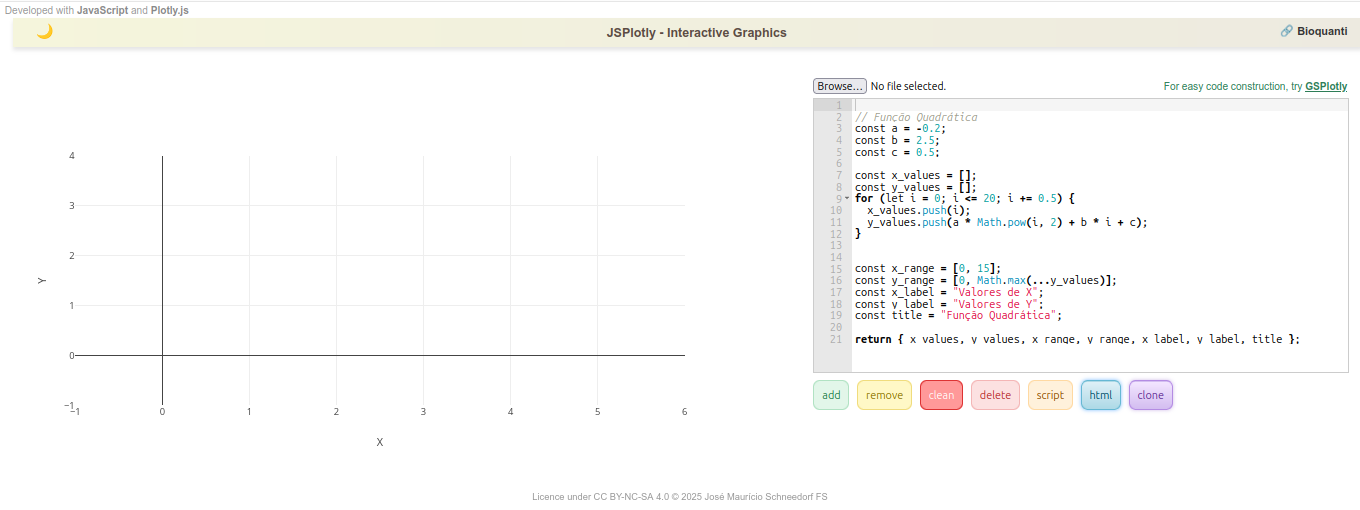
\includegraphics[keepaspectratio]{figs/tela.png}}

}

\caption{\label{fig-tela}Tela única do \emph{JSPlotly}, apresentando o
ecrã gráfico à esquerda e o editor de códigos Ace à direita.}

\end{figure}%

\section{Estrutura do aplicativo}\label{estrutura-do-aplicativo}

~~Observe que o aplicativo é dividido entre uma \emph{área gráfica}
(esquerda) e um \emph{editor de códigos} com alguns botões (direita).A
área de códigos serve para o que naturalmente se apresenta: digitar,
colar, ou editar códigos. A área gráfica apresenta a interpretação da
linguagem para esses códigos. Os comandos são introduzidos por
\href{https://developer.mozilla.org/pt-BR/docs/Web/JavaScript}{JavaScript
(JS)}, uma linguagem de programação moderna, utilizada por grandes
empresas e \emph{big techs}, e focada na interatividade entre a página
web e o usuário. Diferente de outras linguagens, \emph{JavaScript} não
precisa ser compilada, já que é interpretada a partir de máquinas
homônimas de navegadores comuns (\emph{browser}).

\hfill\break

~~\textbf{{Agora vamos à parte divertida !!!}}

\hfill\break

~~Segue abaixo novamente a mesma tela do \emph{JSPlotly}. Aparentemente
é igual à anterior. Mas quer saber a diferença ? Clique na imagem e você
será direcionado ao aplicativo presente no
\href{https://bioquanti.netlify.app/}{Bioquanti}, um site desenvolvido
para apresentar códigos para conteúdos em ensino superior e básico, e
com vários exemplos de objetos pro \emph{JSPlotly}..

\hfill\break

\begin{figure}

\centering{

\href{https://bioquanti.netlify.app/pt/nivel/superior/jsplotly/jsplotly}{\pandocbounded{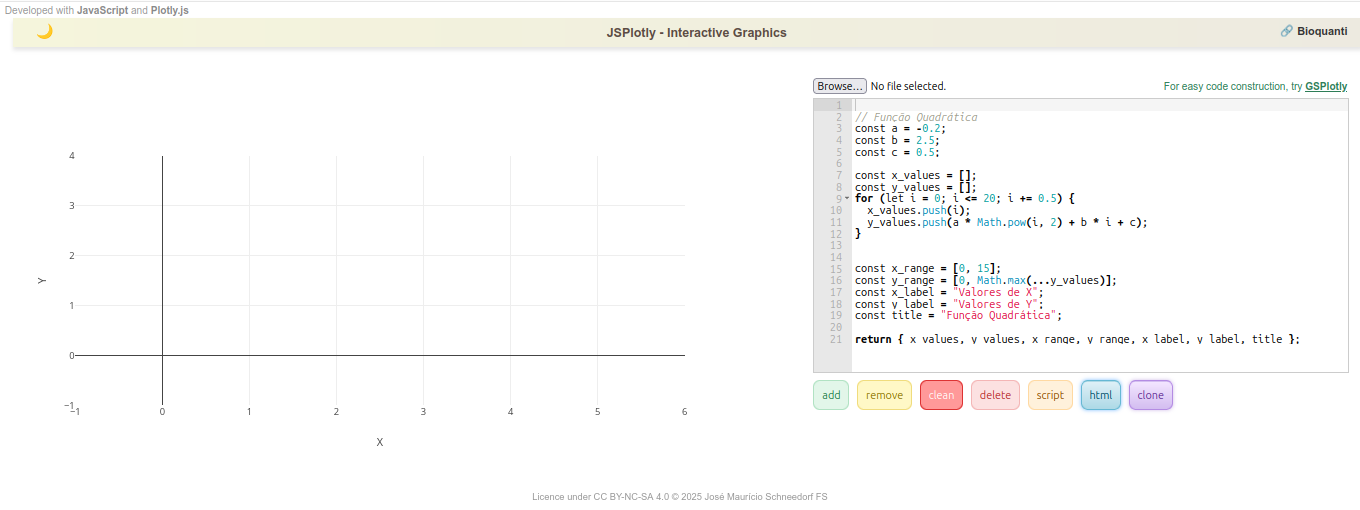
\includegraphics[keepaspectratio]{figs/tela.png}}}

}

\caption{\label{fig-tela}O aplicativo \emph{JSPlotly}, agora ``vivo'' !
Basta clicar na imagem para uma experiência interativa com o app.}

\end{figure}%

\hfill\break

~~O \textbf{aplicativo ``vivo''} pode ser utilizado de forma
independente, armazenado em mídia ou compartilhado facilmente pela web.
Contudo, esse material pretende abordá-lo diretamente em nuvem,
\emph{{misturando texto e programa}}. Nesse caso, estamos falando de
verdadeiros \textbf{{livros vivos}}!!!

\hfill\break

~~Para experimentar esse conceito de \emph{livro vivo}, observe abaixo o
aplicativo \emph{JSPlotly}, inteirinho e funcional, mas desta vez
inserido nesta página web.

\hfill\break

\hfill\break

~~É desta forma que pretende-se abordar os diferentes tópicos com o
programa, ou seja, combinando instruções na página com o próprio
\emph{JSPlotly} e, dessa forma, \emph{``vivificando''} o aprendizado de
temas com o aplicativo.

\hfill\break

~~Bom, seguindo neste tópico sobre a estrutura do aplicativo, passe o
mouse sem clicar em nada na imagem acima, e veja quanta interatividade é
visualizada na mudança do ponteiro do mouse: links para sites na barra
superior (\emph{JavaScript}, \emph{Plotly.js}, \emph{Bioquanti},
\emph{GSPlotly}), ícones acima do gráfico, ícone de claro/escuro no
canto esquerdo, o próprio gráfico, o botão de carregamento de arquivos
(\emph{browse}), o editor de códigos, e os botões abaixo desse.

\hfill\break

\section{\texorpdfstring{Uso do \emph{JSPlotly vivo} na
página}{Uso do JSPlotly vivo na página}}\label{uso-do-jsplotly-vivo-na-puxe1gina}

~~Segue novamente o aplicativo, agora pra você experimentar algumas
ações.

\hfill\break

\hfill\break

~~Observe que há um código \emph{JS} no editor, contendo linhas de
comando. Clique no botão \emph{``add''} abaixo do editor e veja que
surge um gráfico de parábola. Esse gráfico, assim como todos os objetos
produzidos com o \emph{JSPlotly} são \emph{interativos.} Isto quer dizer
que você pode \emph{interagir} com o objeto produzido, no caso o
gráfico. Essa interatividade do objeto é garantida por uma biblioteca
específica desenvolvida em \emph{JavaScript},
\href{https://plotly.com/javascript/}{Plotly.js}.

~~Bibliotecas (ou pacotes) são conjuntos de códigos que, quando
inseridos num algoritmo, permitem automatizar tarefas dentro de uma
linguagem de programação, e sem a necessidade de escrevê-las ``do
zero''. Há diversas bibliotecas para \emph{JavaScript}, algumas
utilizadas no \emph{JSPlotly}, como
\href{https://tonejs.github.io/}{tone.js} para sons e
\href{https://p5js.org/}{p5.js} para objetos multimídia.

\hfill\break

\subsection{\texorpdfstring{Redimensionando a página para conforto
visual do
\emph{JSPlotly}}{Redimensionando a página para conforto visual do JSPlotly}}\label{redimensionando-a-puxe1gina-para-conforto-visual-do-jsplotly}

~~Observe que o aplicativo apresenta-se junto à barra lateral, o que
acaba causando sua redução visual e mesmo omissão de alguns detalhes.
Para melhor conforto e trabalho com o \emph{JSPlotly}, você pode
\textbf{{clicar no ícone do canto superior esquerdo da página}}, próximo
ao título deste capítulo, experimentará o encolhimento da \textbf{barra
lateral}, e consequente readequação visual do \emph{JSPlotly}. Assim,
poderá ajustar como deseja que o \emph{JSPlotly} seja apresentado. Isso
é útil quando se quer explorar o aplicativo visualizando-o de modo mais
confortável.

~~Adicionalmente, a disposição esquerda/direita também adequa-se ao tipo
de dispositivo utilizado. Se for um celular, por exemplo, ela poderá
mudar para cima/embaixo, bastando-se colocá-lo na vertical, ou
esquerda/direita se o dispositivo ficar na horizontal (com permissão
para girar a tela, claro).

\hfill\break

\bookmarksetup{startatroot}

\chapter{Interatividade}\label{interatividade}

\section{\texorpdfstring{Interatividade por mouse, \emph{touchpad}, ou
tela
capacitiva}{Interatividade por mouse, touchpad, ou tela capacitiva}}\label{interatividade-por-mouse-touchpad-ou-tela-capacitiva}

~~Há diversas formas de interagir com o aplicativo e os objetos gerados
por esse, grande parte mediada por mouse em desktop/notebook, por telas
capacitivas de \emph{smartphones}. Ilustrando para uso do mouse,
voltemos ao exemplo da parábola abaixo. Depois de clicar no botão
\emph{add}, experimente:

\begin{Shaded}
\begin{Highlighting}[]
\FloatTok{1.}\NormalTok{ Passar o mouse sobre os pontos do gráfico (}\StringTok{"mouse over"}\NormalTok{ ou }\StringTok{"hover"}\NormalTok{);}
\FloatTok{2.}\NormalTok{ Desenhar um retângulo em qualquer área para ampliação (}\StringTok{"zoom"}\NormalTok{); retorna}\SpecialCharTok{{-}}\NormalTok{se ao tamanho original com um duplo clique;}
\FloatTok{3.}\NormalTok{ Usar o }\StringTok{"zoom"}\NormalTok{ com o botão de rolagem do mouse;}
\FloatTok{4.}\NormalTok{ Escrever qualquer coisa nos rótulos do gráfico, como o título, a etiqueta do eixo das }\FunctionTok{abscissas}\NormalTok{ (eixo }\StringTok{"X"}\NormalTok{), e das }\FunctionTok{ordenadas}\NormalTok{ (eixo }\StringTok{"Y"}\NormalTok{);}
\FloatTok{5.}\NormalTok{ Deslocar o gráfico na horizontal}\SpecialCharTok{/}\NormalTok{vertical, posicionando o mouse próximo dos algarismos de cada eixo, clicando}\SpecialCharTok{{-}}\NormalTok{se com o botão esquerdo, e arrastando}\SpecialCharTok{{-}}\FunctionTok{o}\NormalTok{ (}\StringTok{"pan"}\NormalTok{);}
\end{Highlighting}
\end{Shaded}

\hfill\break

\hfill\break

\section{Botões da barra de modos}\label{botuxf5es-da-barra-de-modos}

~~Além dessa interatividade básica, o \emph{JSPlotly} permite várias
outras, como a promovida pelos botões da barra de modos (\emph{modeBar})
logo acima do gráfico, e identificada pelos ícones a seguir:

\hfill\break


\includegraphics[width=0.7\linewidth,height=\textheight,keepaspectratio]{figs/modebar.png}\\

~~Da direita para a esquerda os ícones permitem:

\begin{Shaded}
\begin{Highlighting}[]
\FloatTok{1.}\NormalTok{ Inserir um texto próximo de um dado do gráfico, e indicado por uma seta;}
\FloatTok{2.}\NormalTok{ Trocar a cor do traço do gráfico;}
\FloatTok{3.}\NormalTok{ Salvar o gráfico como }\FunctionTok{PNG}\NormalTok{ (imagem rasterizada, bom pra web) ou }\FunctionTok{SVG}\NormalTok{ (imagem vetorial, mais precisa);}
\FloatTok{4.}\NormalTok{ Indicar as coordenadas }\StringTok{"x"}\NormalTok{ e }\StringTok{"y"}\NormalTok{ de cada ponto no gráfico por linha tracejada;}
\FloatTok{5.}\NormalTok{ Autoescalonar o gráfico;}
\FloatTok{6.}\NormalTok{ Inserir um círculo;}
\FloatTok{7.}\NormalTok{ Inserir um quadrado;}
\FloatTok{8.}\NormalTok{ Desenhar à mão livre;}
\FloatTok{9.}\NormalTok{ Desenhar uma reta;}
\FloatTok{10.}\NormalTok{ Deslocar o gráfico na área por }\StringTok{"span"}\NormalTok{;}
\FloatTok{11.}\NormalTok{ Aplicar um }\StringTok{"zoom"}\NormalTok{;}
\FloatTok{12.}\NormalTok{ Direcionar o gráfico pra edição detalhada por cliques de mouse no site do desenvolvedor, }\StringTok{"Chart Studio"}\NormalTok{ (https}\SpecialCharTok{:}\ErrorTok{//}\NormalTok{chart}\SpecialCharTok{{-}}\NormalTok{studio.plotly.com}\SpecialCharTok{/}\NormalTok{create}\SpecialCharTok{/}\NormalTok{)}
\end{Highlighting}
\end{Shaded}

\section{Botões do editor de
códigos}\label{botuxf5es-do-editor-de-cuxf3digos}

~~Agora uma explicação sobre os botões abaixo do editor de códigos. São
7 botões, para simplificar o carregamento, cópia e compartilhamento,
tanto do gráfico interativo, como do código que se encontra no editor,
como também para ambos. E até mesmo para o aplicativo em si,
personalizado para um determinado código.

~~O quadro a seguir mostra o que faz cada botão, com detalhes de uso
explicado logo em seguida. Mais uma vez, vamos usar a boa e velha
parábola como exemplo pra você experimentar a funcionalidade de cada
botão.

~~Ah, sim ! Relembrando, os botões sempre aparecem abaixo do editor de
códigos. Mas a disposição do \emph{JSPlotly} pode variar entre
equipamentos. Exemplificando, os botões podem aparecer espalhados abaixo
do editor que fica à direita do gráfico, ou empilhados embaixo do
editor, por sua vez abaixo do gráfico. Isso depende de qual equipamento
você está utilizando para o \emph{JSPlotly}, se um desktop de mesa,
notebook, tablet ou smartphone, e mesmo o nível de \emph{zoom} da tela
do navegador.

~~Quer testar essa disposição num mesmo dispositivo ? Basta clicar no
\emph{botão central superior} que esconde/mostra a barra lateral. E se
estiver usando um celular, Experimente !

\begin{Shaded}
\begin{Highlighting}[]
\CommentTok{\# Botões de funcionalidades do JSPlotly:}

\SpecialCharTok{{-}} \StringTok{"add"}\SpecialCharTok{:}\NormalTok{ adiciona um objeto na área gráfica a partir do código contido no }
\NormalTok{   editor;}
\SpecialCharTok{{-}} \StringTok{"remove"}\SpecialCharTok{:}\NormalTok{ apaga o último traço de um gráfico}\SpecialCharTok{/}\NormalTok{objeto;}
\SpecialCharTok{{-}} \StringTok{"clean"}\SpecialCharTok{:}\NormalTok{ limpa a área gráfica;}
\SpecialCharTok{{-}} \StringTok{"delete"}\SpecialCharTok{:}\NormalTok{ limpa o editor de códigos;}
\SpecialCharTok{{-}} \StringTok{"script"}\SpecialCharTok{:}\NormalTok{ salva o código em formato de texto;}
\SpecialCharTok{{-}} \StringTok{"html"}\SpecialCharTok{:}\NormalTok{ salva o objeto como arquivo HTML, preservando sua interatividade;}
\SpecialCharTok{{-}} \StringTok{"clone"}\SpecialCharTok{:}\NormalTok{ copia o código em sua última edição juntamente com próprio JSPlotly}
\end{Highlighting}
\end{Shaded}

\hfill\break

~~E dá-lhe a parábola pra você testar os botões do editor\ldots.

\hfill\break

\hfill\break

\subsection{\texorpdfstring{Botão
\emph{add}}{Botão add}}\label{botuxe3o-add}

~~O botão \emph{add} é o principal do editor. Com ele você adiciona o
código no interpretador de \emph{JavaScript} do navegador,
possibilitando a construção do gráfico (ou de outro objeto interativo,
como veremos adiante). Agora, o botão \emph{add} possui outra função bem
bacana, e que você pode experimentar nesse momento com 2 cliques:

\hfill\break

\begin{enumerate}
\def\labelenumi{\arabic{enumi}.}
\tightlist
\item
  Clique no \emph{add} do editor para adicionar a parábola;
\item
  Apague o sinal de \emph{``-''} que está logo acima no código, na
  variável \emph{``const a = -0.2''};
\item
  Clique novamente no botão \emph{add}.\\
\end{enumerate}

~~Tchan, tchan, tchaaan !!! Veja que agora o gráfico
\emph{``(add)icionou''} mais um traço ao gráfico original. E ainda por
cima com cor diferente e legenda !!

\hfill\break

\begin{figure}

\centering{

\pandocbounded{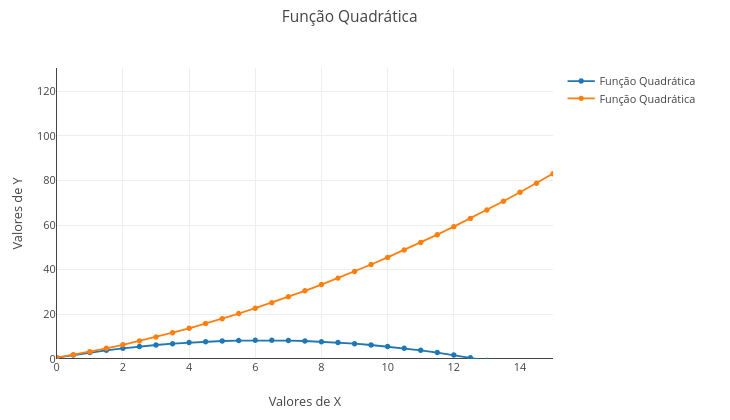
\includegraphics[keepaspectratio]{figs/addParabola.png}}

}

\caption{\label{fig-addParabola}Gráfico de parábola sobrepondo a equação
original à sua alteração na constante ``a'' (retirada do sinal
negativo).}

\end{figure}%

\hfill\break

~~E para dar um jeitão mais bacana ao gráfico, dá-lhe outra
funcionalidade interativa: a legenda. Veja que você pode clicar e
arrastar a legenda para outra parte do gráfico. Além disso, também pode
mudar o texto legenda, já que o gráfico sobreposto possui o mesmo título
do anterior. Exemplificando:

\hfill\break

\begin{enumerate}
\def\labelenumi{\arabic{enumi}.}
\tightlist
\item
  Clique no texto em azul na legenda e digite \emph{``a = - 0,2''};
\item
  Agora clique no texto em laranja e digite \emph{``a = 0,2''}
\end{enumerate}

~~Pronto, agora você tem um gráfico mais \emph{``limpinho''} na legenda,
como no debaixo.

\begin{figure}

\centering{

\pandocbounded{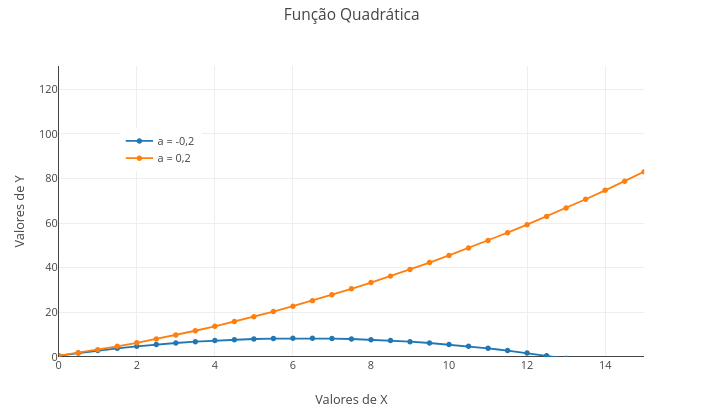
\includegraphics[keepaspectratio]{figs/addParabola_legenda.png}}

}

\caption{\label{fig-addParabola_legenda}Gráfico de parabóla
personalizado com edição de texto direto na legenda e o reposicionamento
dessa com clique/arraste por mouse.}

\end{figure}%

\hfill\break

~~Essa possibilidade com o botão \emph{add} para adicionar traços é
particularmente interessante quando se deseja comparar um gráfico (ou
objeto) com outro, para se verificar o que mudou na área gráfica com a
alteração do código. Ou seja, isso é muito bom pra explorar parâmetros
de uma equação, por exemplo, com vistas a compreender melhor como essa
equação funciona quando colocada na forma de um gráfico. O nome chique
pra isso é \emph{exploração ou manipulação paramétrica}. Em resumo,
elabora-se um gráfico e o sobrepõe com um ou mais gráficos alterando-se
um ou mais parâmetros da equação. No caso de um objeto diferente de um
gráfico, a exploração dá-se com mudança de outros detalhes do código
(com cores, por exemplo).

\subsection{\texorpdfstring{Botão
\emph{remove}}{Botão remove}}\label{botuxe3o-remove}

~~Tá em inglês, mas poderia tranquilamente ser compreendido em língua
pátria, mesmo. Esse botao remove o último traço adicionado na área
gráfica. Sua utilidade é também importante, pois permite que se retire
de um gráfico um ou mais traços que não ficaram do jeito que se
desejava. Exemplificando, digamos que para a parábola do exemplo acima o
legal seria comparar o efeito da constante \emph{``a''} com um valor que
não fosse somente pela retirada do sinal negativo. A figura abaixo
ilustra como ficaria o gráfico se você \emph{``(remove)''esse} esse
traço e adicionasse outro, com valor diferente para a constante.

\begin{figure}

\begin{minipage}{0.33\linewidth}

\centering{

\pandocbounded{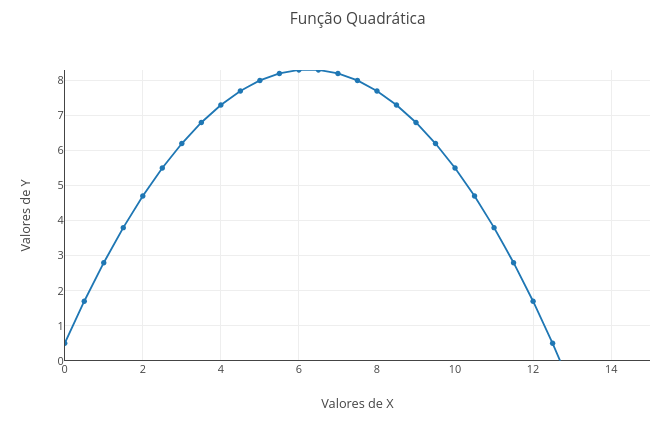
\includegraphics[keepaspectratio]{figs/remove1.png}}

}

\subcaption{\label{fig-remove1}Parábola com o código original, e \emph{a
= -0.2}.}

\end{minipage}%
%
\begin{minipage}{0.33\linewidth}

\centering{

\pandocbounded{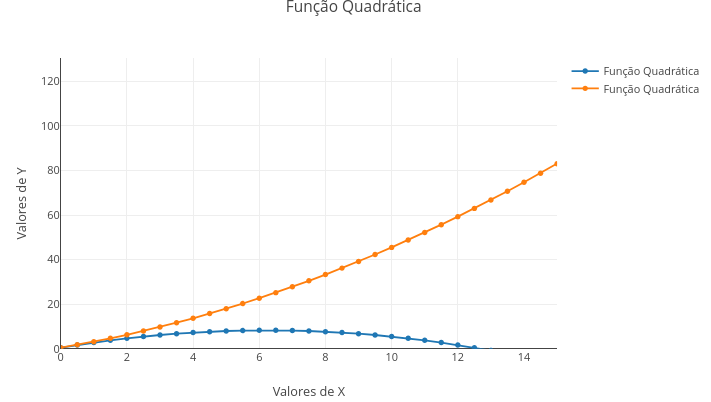
\includegraphics[keepaspectratio]{figs/remove2.png}}

}

\subcaption{\label{fig-remove2}Parábola com adição de traço para \emph{a
= 0.2}.}

\end{minipage}%
%
\begin{minipage}{0.33\linewidth}

\centering{

\pandocbounded{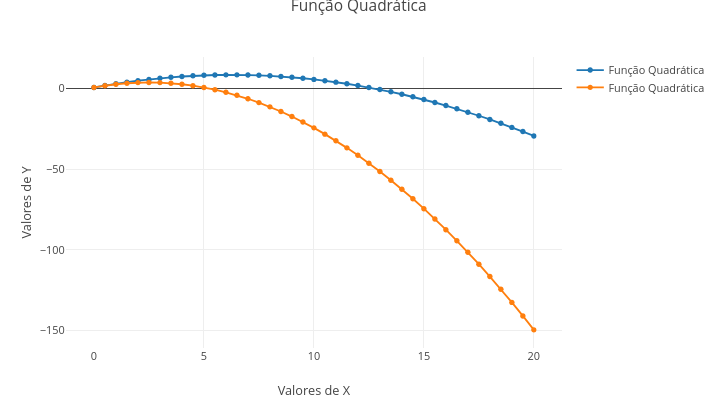
\includegraphics[keepaspectratio]{figs/remove3.png}}

}

\subcaption{\label{fig-remove2}Parábola para remoção do traço anterior
(\emph{remove}) e nova adição de traço (\emph{add}), dessa vez com
\emph{a = -0.5}.}

\end{minipage}%

\caption{\label{fig-comparaParabola}Sequência de gráficos de parábolas
para exemplificar o uso do botão \emph{add} para inserção e
\emph{remove} para remoção de traços.}

\end{figure}%

\hfill\break

\subsection{\texorpdfstring{Botões \emph{clean} e
\emph{delete}}{Botões clean e delete}}\label{botuxf5es-clean-e-delete}

~~Esses botões servem para limpeza. O botão \emph{clean} atua limpando a
área gráfica. Pode ser que às vezes \emph{``sobre''} alguns elementos de
interatividade de um gráfico anterior, como uma barra deslizante, por
exemplo. Nesse caso, o melhor é recarregar a tela do navegador (Ctrl+F5
ou Ctrl+R, dependendo do \emph{browser}, ou um botão à esquerda de sua
barra de endereços).

~~Já o botão \emph{delete} limpa o editor de códigos, o que pode ser
útil quando se deseja colar aí um novo código, por exemplos.

\hfill\break

\subsection{\texorpdfstring{Botão
\emph{script}}{Botão script}}\label{botuxe3o-script}

~~Esse botão permite que você salve o código para recuperá-lo
futuramente, para editá-lo num outro momento, ou para compartilhá-lo com
alguém. Ele é salvo com o atributo \emph{js} indicando tratar-se de um
código em \emph{JavaScript} para carregamento no \emph{JSPlotly} pelo
botão \emph{browser}. Mas você pode personalizar o nome, e abri-lo em
qualquer editor de texto, mesmo num simples bloco de notas.

~~O botão é particularmente útil quando se deseja compartilhar o código,
e mesmo guardá-lo para um uso futuro, para montar uma biblioteca e
códigos, ou para instruir um assistente de IA generativa para
incrementar o código, ou produzir um código semelhante.

\hfill\break

\subsection{\texorpdfstring{Botão
\emph{html}}{Botão html}}\label{botuxe3o-html}

~~Esse botão é o \emph{``mais charmoso''}. O \emph{html} permite que
você salve o gráfico ou qualquer outro objeto interativo num arquivo
HTML, por óbvio. Mas o ``\emph{chique da coisa''} é que o arquivo é
\emph{autossuficiente} (\emph{self-contained}). Na prática isso quer
dizer que ele guarda toda a interatividade contida no objeto interativo
original, incluindo ações de mouse/dedo, animações, sonorização, e
\emph{widgets}.

~~Assim, você pode rodar um código e, apreciado o objeto que resulta
desse, salvá-lo numa mídia física para uso pessoal, estudo futuro,
armazenamento simples, como também para distribui-lo a quem desejar,
incluindo o seu compartilhamento por redes sociais ! Que tal
experimentar isso agora ?!

~~Com a boa velha parábola (código padrão que vem com o \emph{JSPlotly})
do aplicativo \emph{vivo} abaixo:

\begin{enumerate}
\def\labelenumi{\arabic{enumi}.}
\tightlist
\item
  Clique em \emph{add} para adicionar o gráfico, como já fez antes;
\item
  Passe o mouse na área gráfica (ou os dedos no \emph{touchpad} do
  notebook, ou na tela capacitiva do celular), e clique em algum ícone
  da \emph{barra de modos} (o de câmera, por exemplo, pra mudar a cor do
  traço);
\item
  Clique em \emph{html} e salve o arquivo no dispositivo (notebook,
  celular, etc).
\item
  Abra o arquivo salvo e veja que ele retém toda a interatividade do
  objeto, incluindo a personalização realizada (cor do traço, por ex);
\end{enumerate}

\hfill\break

~~Só pra te mostrar como fica, veja a imagem abaixo, uma
\emph{{representação viva do que faz o botão html}}. Basta clicar na
imagem para acessar a velha e boa parábola que vem como padrão no
\emph{JSPlotly}, mas como um arquivo interativo pronto pra estudo ou
compartilhamento !

\begin{figure}

\centering{

\href{figs/htmlVivo.html}{\pandocbounded{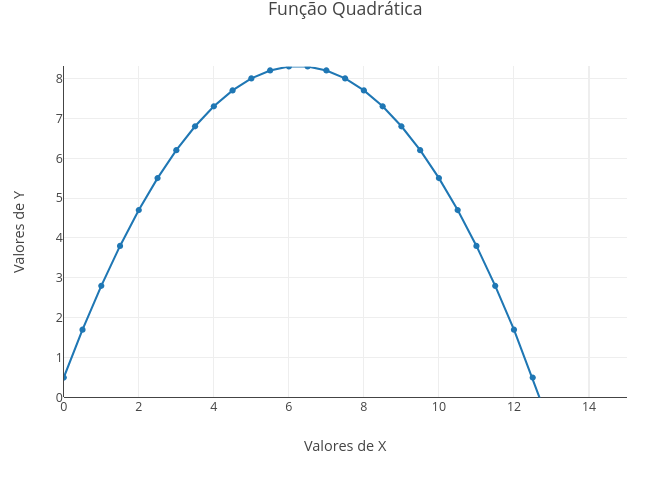
\includegraphics[keepaspectratio]{figs/parabola.png}}}

}

\caption{\label{fig-tela}A parábola \emph{viva}, tal como armazenada
pelo botão \emph{html}.}

\end{figure}%

\subsection{\texorpdfstring{Botão
\emph{clone}}{Botão clone}}\label{botuxe3o-clone}

~~Esse botão é o mais \emph{disruptivo}, como se diz nesses tempos. O
\emph{clone} cumpre a função que seu nome apresenta, ou seja, ele
\emph{``clona''} o \emph{JSPlotly} com um código específico, já
customizado ou não. Isso é particularmente útil quando se quer não
apenas guardar/compartilhar um código (botão \emph{script}) ou um objeto
interativo (botão \emph{html}), mas sim quando se deseja
guardar/compartilhar o aplicativo inteiro com o código padrão escolhido
e já customizado.

~~Dessa forma, o botão \emph{clone} agrega um valor a mais, já que
possibilita trabalhar com um objeto interativo juntamente com seu
código, facultando a edição desse para personalização do objeto.
Ilustrando seu uso prático, quando se deseja guardar/compartilhar um
objeto e seu código para aprimoramento, por exemplo. Bom, como o
\emph{clone} \emph{``clona''} um gráfico com seu código junto ao
aplicativo, não teria a menor graça reproduzir \emph{``mais do mesmo''}
aqui !

\bookmarksetup{startatroot}

\chapter{Bot de IA para códigos}\label{bot-de-ia-para-cuxf3digos}

~~Como visto nas seções anteriores, o \emph{JSPlotly} trabalha com
códigos de programação ! São comandos escritos em linguagem
\emph{JavaScript}, a qual é interpretada junto a máquinas homônimas de
navegadores modernos (ex: Chrome, Firefox, Safari, Opera, Edge, etc).
Agora\ldots convenhamos\ldots além de amantes das \emph{Ciências da
Computação}, quem gosta de códigos de programação ?!

~~Pensando nisso foi desenvolvido junto ao aplicativo um \emph{gerador
de códigos pro JSPlotly por assistente de inteligência artificial (IA)}
!!! Isso quer dizer que {\textbf{você não precisa saber nada sobre
programação !!!}}.

\hfill\break

~~Quer fazer o um teste ?

\hfill\break

~~Clique no link do
\href{https://chatgpt.com/g/g-6819fbb8d2d08191bf7d50a3dbeadb0d-gsplotly?model=gpt-4o}{GSPlotly}
(\emph{G} para \emph{gerador}) ou na imagem abaixo, e peça ao gerador
para construir alguma coisa\ldots digamos\ldots.

~~{\ldots{}``faça um gráfico de barras sobre as principais regiões de
terras raras''\ldots{}}

\hfill\break

\begin{figure}

\centering{

\href{https://chatgpt.com/g/g-6819fbb8d2d08191bf7d50a3dbeadb0d-gsplotly}{\pandocbounded{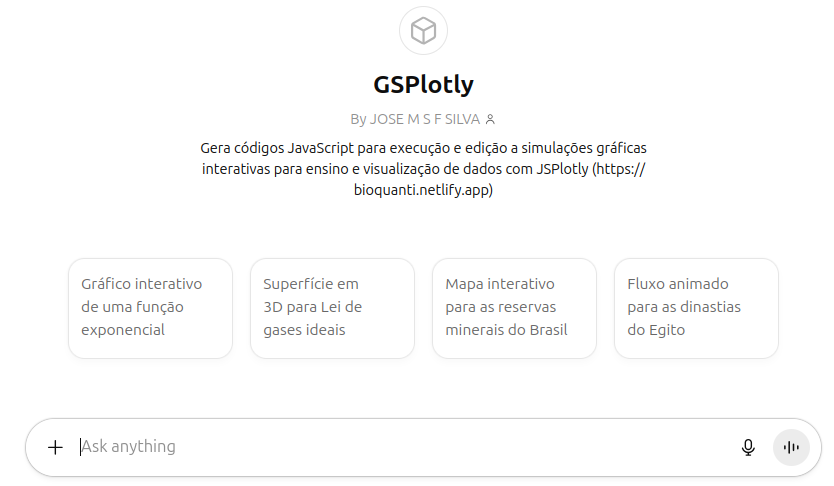
\includegraphics[keepaspectratio]{figs/gsplotly.png}}}

}

\caption{\label{fig-gsplotly}Tela do \emph{GSPlotly} para criação de
códigos ao simulador JSPlotly. Clique na imagem para acessar o gerador!}

\end{figure}%

\hfill\break

~~Observe que o \emph{GSPlotly} fornece o código \emph{JavaScript} quase
que instantaneamente, e ainda por cima dá algumas dicas pra melhoria do
próprio código !

~~Agora é só copiar o código pelo ícone que aparece no canto superior
direito (\emph{``copy code''}) e rodar no \emph{JSPlotly}. Para isso:

\begin{enumerate}
\def\labelenumi{\arabic{enumi}.}
\tightlist
\item
  Copie o código;
\item
  Clique em \emph{delete} no \emph{JSPlotly} abaixo;
\item
  Cole o código;
\item
  Clique em \emph{add}.
\end{enumerate}

\hfill\break

~~Se deu tudo certo, você deverá ver algo parecido com a imagem
\emph{interativa} abaixo:

\hfill\break

\begin{figure}

\centering{

\href{figs/terrasraras.html}{\pandocbounded{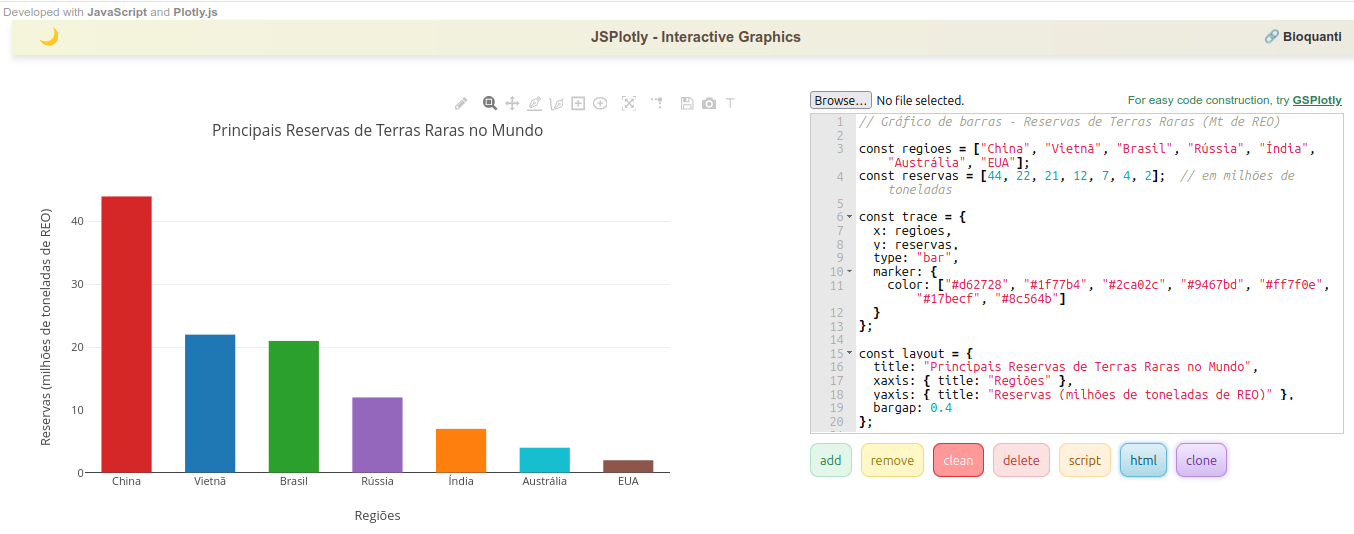
\includegraphics[keepaspectratio]{figs/terrasraras.png}}}

}

\caption{\label{fig-terrasraras}\emph{JSPlotly} interativo contendo o
código para a construção de um gráfico de barras para reservas mundiais
de terras raras, tal como sugerido acima ao gerador \emph{GSPlotly} de
IA.}

\end{figure}%

\section{\texorpdfstring{Algumas dicas para uma \emph{``boa conversa''}
com o
\emph{GSPlotly}}{Algumas dicas para uma ``boa conversa'' com o GSPlotly}}\label{algumas-dicas-para-uma-boa-conversa-com-o-gsplotly}

~~Elaborar um gráfico, mapa, animação, simulação, sonorização, e mesmo
um game inteiro no \emph{JSPlotly} com auxílio de um bot de IA como o
\emph{GSPlotly} é plenamente possível (vide os objetos virtuais
disponíveis para
\href{https://bioquanti.netlify.app/pt/nivel/basico/jsplotly/jsplotly_bas}{ensino
básico} ou
\href{https://bioquanti.netlify.app/pt/nivel/superior/jsplotly/jsplt_bioq}{ensino
superior} no site \emph{Bioquanti}). Contudo, há objetos virtuais mais
simples (um gráfico, por exemplo) e mais complexos (um objeto
multimídia, por exemplo) e, para isso, faz-se necessário um \emph{``toma
lá dá cá''} entre você e o assistente de IA, dependendo do grau de
complexidade do objeto virtual pretendido.

~~Algumas rápidas orientações para que essa comunicação ou
\emph{engenharia de prompts} seja eficiente são sugeridas abaixo.

\begin{Shaded}
\begin{Highlighting}[]
\FloatTok{1.}\NormalTok{ Fundamentalmente, não desista da }\DecValTok{1}\NormalTok{a. vez }\SpecialCharTok{!!}\NormalTok{ Por vezes a IA não entrega o que se deseja de primeira, exigindo uma troca de informações entre o usuário e o bot para que se atinja o objetivo do primeiro;}

\FloatTok{2.}\NormalTok{ Se a IA não lhe devolver o que deseja nas primeiras tentativas, comece com algo mais simples;}

\FloatTok{3.}\NormalTok{ Se mesmo o simples não resolver, reduza a complexidade do pedido. Separe o problema em partes, e tente a solução para a parte mais básica do problema; só depois de }\FunctionTok{conquistada}\NormalTok{ (testada no JSPlotly), solicite à IA a solução para uma nova parte a acrescentar junto a que foi bem }\FunctionTok{sucedida.}\NormalTok{ (sem trocadilhos, isso é }\StringTok{"parte"}\NormalTok{ do chamado }\StringTok{"pensamento computacional"}\NormalTok{...ou....}\StringTok{"dividir para conquistar"}\SpecialCharTok{!}\NormalTok{);}

\FloatTok{4.}\NormalTok{ Experimente oferecer o código que ainda não está a seu gosto para outro assistente de IA, para correção ou melhorias. Você pode fazê}\SpecialCharTok{{-}}\NormalTok{lo simplesmente copiando o código e colando}\SpecialCharTok{{-}}\NormalTok{o no outro bot de IA, ou por carregamento nesse após salvá}\SpecialCharTok{{-}}\NormalTok{lo como arquivo no JSPlotly com o botão }\StringTok{"script"}\NormalTok{.}

\FloatTok{5.}\NormalTok{ Aprenda a conhecer linguagem aos poucos. Isso lhe dará maior autonomia e segurança, tanto pra lidar com bots de IA, como para corrigir e aprimorar códigos }\StringTok{"sem auxílio da IA"}\NormalTok{. E mesmo para }\StringTok{"desenvolver novos códigos sozinho"} \SpecialCharTok{!!!}
\end{Highlighting}
\end{Shaded}




<button id="sb-toggle" class="btn btn-light" title="Sidebar" aria-label="Sidebar">
  <i class="bi bi-layout-text-sidebar-reverse"></i>
</button>

<style>
  /* Botão fixo: não interfere no layout */
  #sb-toggle{
    position: fixed; top: 12px; left: 12px; z-index: 10000;
    border-radius: 999px; padding: 8px 10px; box-shadow: 0 4px 10px rgba(0,0,0,.15);
  }

  /* Quando a classe estiver no body, sumir com sidebars e ocupar largura total */
  body.sb-hidden #quarto-sidebar,
  body.sb-hidden #quarto-sidebar-glass,
  body.sb-hidden #quarto-margin-sidebar { display: none !important; }

  /* Grid do Quarto: faz o main ocupar tudo quando sidebar está oculta */
  body.sb-hidden .page-columns { grid-template-columns: 1fr !important; }
  body.sb-hidden main.content { grid-column: 1 / -1 !important; }
</style>

<script type="module">
  const BODY = document.body;
  const btn  = document.getElementById('sb-toggle');

  // restaura preferência
  if (localStorage.getItem('sb-hidden') === '1') BODY.classList.add('sb-hidden');

  const sync = () => localStorage.setItem('sb-hidden', BODY.classList.contains('sb-hidden') ? '1' : '0');

  btn?.addEventListener('click', () => { BODY.classList.toggle('sb-hidden'); sync(); });

  // atalho S (fora de inputs)
  document.addEventListener('keydown', ev => {
    if (ev.key.toLowerCase() === 's' && !ev.target.closest('input, textarea, [contenteditable="true"]')) {
      ev.preventDefault(); btn.click();
    }
  });

  // se o botão nativo do Quarto existir, manter estados sincronizados
  const hdrBtn = document.querySelector('header .quarto-btn-toggle');
  hdrBtn?.addEventListener('click', () => setTimeout(sync, 200));
</script>


\end{document}
